\documentclass[11pt,a4paper]{article}
\usepackage[T2A]{fontenc}
\usepackage[utf8]{inputenc}
\usepackage[russian]{babel}
\usepackage{amsmath,amssymb}
\usepackage{geometry}
\usepackage{enumitem}
\usepackage{float}
\geometry{margin=2cm}
\usepackage{graphicx}

\title{М5. Автогенератор на туннельном диоде}
\author{}
\date{}

\begin{document}
\maketitle

\section{Постановка задачи}
Рассматривается электрическая схема автогенератора:
\begin{figure}[H]
    \centering
    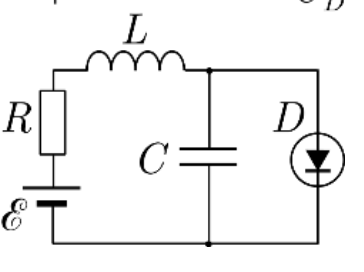
\includegraphics[width=0.5\linewidth]{image.png}
    \label{fig:placeholder}
\end{figure}

\section{ВАХ туннельного диода}
По условию, при $U_D>0$:
\begin{equation}
I_D(U_D)=aU_D^3+bU_D^2+cU_D,\qquad I_D(U_D)=0\ \text{при}\ U_D\le 0.
\end{equation}
Коэффициенты (в СИ):
\[
a=4\cdot 10^{-3}\,\frac{A}{V^3},\qquad
b=-16\cdot 10^{-3}\,\frac{A}{V^2},\qquad
c=17\cdot 10^{-3}\,\frac{A}{V}.
\]

\subsection{Дифференциальная проводимость}
Дифференциальная проводимость диода:
\begin{equation}
g_D(U)=\frac{dI_D}{dU}=3aU^2+2bU+c \qquad (U>0).
\end{equation}
Область отрицательной проводимости определяется условием $g_D(U)<0$.
Для заданных $a,b,c$ нули $g_D(U)$:
\[
U_1\approx 0.732\ \text{В},\qquad U_2\approx 1.934\ \text{В},
\]
и, следовательно,
\[
g_D(U)<0 \quad \text{при}\quad U\in(U_1,U_2)\approx(0.73;1.93)\ \text{В}.
\]

\section{Вывод уравнений модели (законы Кирхгофа)}
Обозначим напряжение на диоде/конденсаторе как $U(t)$, ток через индуктивность (и резистор) как $I(t)$.

\subsection{2-й закон Кирхгофа (закон напряжений) для последовательной ветви}
Падения напряжений на $R$ и $L$ и на узле $U(t)$ суммируются и равны ЭДС:
\begin{equation}
\varepsilon = RI + L\frac{dI}{dt} + U.
\end{equation}
Отсюда:
\begin{equation}
L\frac{dI}{dt} = \varepsilon - RI - U.
\end{equation}

\subsection{1-й закон Кирхгофа (закон токов) для узла}
Ток $I$ делится на ток через конденсатор и через диод:
\begin{equation}
I = I_C + I_D(U),\qquad I_C=C\frac{dU}{dt}.
\end{equation}
Отсюда:
\begin{equation}
C\frac{dU}{dt} = I - I_D(U).
\end{equation}

\subsection{Итоговая система ОДУ}
\begin{equation}
\boxed{
\begin{aligned}
L\frac{dI}{dt} &= \varepsilon - RI - U,\\
C\frac{dU}{dt} &= I - I_D(U).
\end{aligned}}
\end{equation}
Это стандартная модель автогенератора с нелинейным элементом.

\section{Равновесие и линеаризация (критерий автогенерации)}
\subsection{Точка равновесия}
В равновесии $\dot I=\dot U=0$:
\begin{equation}
I_0=I_D(U_0),\qquad \varepsilon = RI_0 + U_0.
\end{equation}
То есть рабочая точка $(U_0,I_0)$ --- пересечение нагрузочной прямой $I=(\varepsilon-U)/R$ с ВАХ $I_D(U)$.

\subsection{Линеаризация}
Пусть $U=U_0+u$, $I=I_0+i$, где $u,i$ малы. Разложим ток диода:
\[
I_D(U_0+u)\approx I_D(U_0)+g_0u,\qquad g_0=g_D(U_0).
\]
Тогда линейная система:
\begin{equation}
\begin{aligned}
L\dot i &= -Ri-u,\\
C\dot u &= i-g_0u.
\end{aligned}
\end{equation}
Исключая $i$, получаем уравнение второго порядка для $u(t)$:
\begin{equation}
\boxed{
LC\,\ddot u + (RC+Lg_0)\,\dot u + (1+Rg_0)\,u = 0.}
\end{equation}

\subsection{Критерий возникновения автоколебаний}.

\textbf{условие самовозбуждения}:
\begin{equation}
\boxed{RC + Lg_0 < 0 \quad \Longleftrightarrow\quad g_0 < -\frac{RC}{L}.}
\end{equation}

\textbf{В терминах дифференциального сопротивления} $r_d=\left(\frac{dI}{dU}\right)^{-1}=\frac{1}{g_0}$:
\[
r_d<0,\qquad |r_d|>\frac{L}{RC}.
\]

\subsection{Оценка частоты}
Если затухание мало, то собственная частота близка к:
\begin{equation}
\omega \approx \sqrt{\frac{1+Rg_0}{LC}},\qquad
f\approx \frac{\omega}{2\pi}\approx \frac{1}{2\pi\sqrt{LC}}\ \ (\text{при }|Rg_0|\ll 1).
\end{equation}

\section{Ответы на вопросы}

\subsection{1) При каких параметрах происходит автогенерация?}
\textbf{Автогенерация возникает}, если выполнены два условия:
\begin{enumerate}[leftmargin=6mm]
    \item рабочая точка лежит в области отрицательной дифференциальной проводимости:
    \[
    g_D(U_0)=\left.\frac{dI_D}{dU}\right|_{U_0}<0;
    \]
    \item отрицательная проводимость диода по модулю перекрывает потери в контуре:
    \[
    RC+Lg_D(U_0)<0.
    \]
\end{enumerate}
\[
\boxed{g_D(U_0)<-\frac{RC}{L}.}
\]
\textbf{Эквивалентно через дифференциальное сопротивление}
$r_d(U_0)=\left(\frac{dI_D}{dU}\right)^{-1}$:
\[
\boxed{r_d(U_0)<0,\qquad |r_d(U_0)|>\frac{L}{RC}.}
\]
Если эти условия не выполняются, возмущения затухают и автогенерации нет.

\subsection{2) При каких параметрах генерируется практически чистая синусоида?}
Практически чистая синусоида соответствует режиму слабой нелинейности, когда выполняются:
\[
RC+Lg_D(U_0)\approx 0,\qquad g_D(U_0)<0,
\]
а рабочая частота близка собственной частоте контура:
\[
\omega\approx\frac{1}{\sqrt{LC}}.
\]


\subsection{3) Какова максимальная амплитуда колебаний?}
\textbf{Максимальная амплитуда} установившихся автоколебаний определяется нелинейным энергетическим балансом за период:
\[
W_{\text{подкачка диодом}} = W_{\text{потери на }R}.
\]
В среднем по периоду:
\[
\left\langle U(t)I_D\bigl(U(t)\bigr)\right\rangle
=
\left\langle RI^2(t)\right\rangle.
\]
Значение $U_{\max}$ находится из условия существования предельного цикла (периодического решения нелинейной системы).

\end{document}